\documentclass[nojss]{jss}\usepackage[]{graphicx}\usepackage[]{color}
%% maxwidth is the original width if it is less than linewidth
%% otherwise use linewidth (to make sure the graphics do not exceed the margin)
\makeatletter
\def\maxwidth{ %
  \ifdim\Gin@nat@width>\linewidth
    \linewidth
  \else
    \Gin@nat@width
  \fi
}
\makeatother

\definecolor{fgcolor}{rgb}{0.345, 0.345, 0.345}
\newcommand{\hlnum}[1]{\textcolor[rgb]{0.686,0.059,0.569}{#1}}%
\newcommand{\hlstr}[1]{\textcolor[rgb]{0.192,0.494,0.8}{#1}}%
\newcommand{\hlcom}[1]{\textcolor[rgb]{0.678,0.584,0.686}{\textit{#1}}}%
\newcommand{\hlopt}[1]{\textcolor[rgb]{0,0,0}{#1}}%
\newcommand{\hlstd}[1]{\textcolor[rgb]{0.345,0.345,0.345}{#1}}%
\newcommand{\hlkwa}[1]{\textcolor[rgb]{0.161,0.373,0.58}{\textbf{#1}}}%
\newcommand{\hlkwb}[1]{\textcolor[rgb]{0.69,0.353,0.396}{#1}}%
\newcommand{\hlkwc}[1]{\textcolor[rgb]{0.333,0.667,0.333}{#1}}%
\newcommand{\hlkwd}[1]{\textcolor[rgb]{0.737,0.353,0.396}{\textbf{#1}}}%

\usepackage{framed}
\makeatletter
\newenvironment{kframe}{%
 \def\at@end@of@kframe{}%
 \ifinner\ifhmode%
  \def\at@end@of@kframe{\end{minipage}}%
  \begin{minipage}{\columnwidth}%
 \fi\fi%
 \def\FrameCommand##1{\hskip\@totalleftmargin \hskip-\fboxsep
 \colorbox{shadecolor}{##1}\hskip-\fboxsep
     % There is no \\@totalrightmargin, so:
     \hskip-\linewidth \hskip-\@totalleftmargin \hskip\columnwidth}%
 \MakeFramed {\advance\hsize-\width
   \@totalleftmargin\z@ \linewidth\hsize
   \@setminipage}}%
 {\par\unskip\endMakeFramed%
 \at@end@of@kframe}
\makeatother

\definecolor{shadecolor}{rgb}{.97, .97, .97}
\definecolor{messagecolor}{rgb}{0, 0, 0}
\definecolor{warningcolor}{rgb}{1, 0, 1}
\definecolor{errorcolor}{rgb}{1, 0, 0}
\newenvironment{knitrout}{}{} % an empty environment to be redefined in TeX

\usepackage{alltt}

%%%%%%%%%%%%%%%%%%%%%%%%%%%%%%
%% declarations for jss.cls %%
%%%%%%%%%%%%%%%%%%%%%%%%%%%%%%
%\VignetteEngine{knitr::knitr}
%\VignetteIndexEntry{ggRandomForests}
%\VignetteIndexEntry{A guide to Random Forests with the randomForestSRC and ggRandomForests packages}                                          
%\VignetteKeywords{random forest, survival, classification, regression, VIMP, minimal depth}                                                                   
%\VignetteDepends{ggRandomForests}                                      
%\VignettePackage{ggRandomForests} 

%% almost as usual
\author{John Ehrlinger \and Jeevanantham Rajeswaran
%\\Cleveland Clinic 
%\AND Hemant Ishwaran \\University of Miami
%\And Liang Li\\MD Anderson Cancer Center
%\AND Udaya B. Kogalur 
\and Eugene H. Blackstone\\Cleveland Clinic}

\title{{\pkg{ggRandomForests}}: Visually Exploring Random Forests in \proglang{R}}

%% for pretty printing and a nice hypersummary also set:
\Plainauthor{Ehrlinger et.\ al.\ } %% comma-separated
\Plaintitle{ggRandomForests: Visually Exploring Random Forests} %% without formatting
\Shorttitle{{\pkg{ggRandomForests}}: Visually Exploring Random Forests in \proglang{R}}

%% an abstract and keywords
\Abstract{ 
Random Forests~\citep{Breiman:2001} (RF) are a fully non-parametric statistical method requiring no distributional assumptions on covariate relation to the response. RF are a robust, nonlinear technique that optimizes predictive accuracy by fitting an ensemble of trees to stabilize model estimates. Random Forests for survival~\citep{Ishwaran:2007a,Ishwaran:2008} (RF-S) are an extension of Breiman's RF techniques to survival settings, allowing efficient non-parametric analysis of time to event data. The \pkg{randomForestSRC} package~\citep{Ishwaran:RFSRC:2014} is a unified treatment of Breiman's random forests for survival, regression and classification problems.

Predictive accuracy make RF an attractive alternative to parametric models, though complexity and interpretability of the forest hinder wider application of the method. We introduce the \pkg{ggRandomForests} package, tools for creating and plotting data structures to visually understand random forest models grown in \proglang{R} with the \pkg{randomForestSRC} package. The \pkg{ggRandomForests} package is structured to extract intermediate data objects from \pkg{randomForestSRC} objects and generate figures using the \pkg{ggplot2}~\citep{Wickham2009} graphics package.

Using both classification (RF-C) and survival (RF-S) examples from our research at the Cleveland Clinic, we will demonstrate the \pkg{randomForestSRC} package. We use Variable Importance measure (VIMP)~\citep{Breiman:2001} as well as  Minimal Depth~\citep{Ishwaran:2010}, a property derived from the construction of each tree within the forest, to assess the impact of variables on forest prediction. We will also demonstrate the use of variable dependence plots~\citep{Friedman00greedyfunction} to aid interpretation RF results in different response settings. 
}
\Keywords{random forest, survival, classification, regression, VIMP, minimal depth}
\Plainkeywords{random forest, survival, classification, regression, VIMP, minimal depth}
%% at least one keyword must be supplied

%% publication information
%% NOTE: Typically, this can be left commented and will be filled out by the technical editor
%% \Volume{13}
%% \Issue{9}
%% \Month{September}
%% \Year{2004}
%% \Submitdate{2004-09-29}
%% \Acceptdate{2004-09-29}

%% The address of (at least) one author should be given
%% in the following format:
\Address{
John Ehrlinger\\
Quantitative Health Sciences\\
Lerner Research Institute\\
Cleveland Clinic\\
9500 Euclid Ave\\
Cleveland, Ohio 44195\\
%  Telephone: +41/0/44634-4643 \\
%  Fax: +41/0/44634-4386 \\
E-mail: \email{john.ehrlinger@gmail.com}\\
URL: \url{http://www.lerner.ccf.org/qhs/people/ehrlinj/}
}

%% It is also possible to add a telephone and fax number
%% before the e-mail in the following format:
%% Telephone: +43/1/31336-5053
%% Fax: +43/1/31336-734

%% for those who use Sweave please include the following line (with % symbols):
%% need no \usepackage{Sweave.sty}

%% end of declarations %%%%%%%%%%%%%%%%%%%%%%%%%%%%%%%%%%%%%%%%%%%%%%%



\IfFileExists{upquote.sty}{\usepackage{upquote}}{}
\begin{document}

%% include your article here, just as usual
%% Note that you should use the \pkg{}, \proglang{} and \code{} commands.



% -----------------------------------------------------
\section{About this document}
% -----------------------------------------------------
This document is an introduction to the \pkg{ggRandomForests} \proglang{R} package. 

% -----------------------------------------------------
\section{Introduction} \label{S:introduction}
% -----------------------------------------------------

Random Forests~\citep{Breiman:2001} (RF) are a robust statistical method that utilizes all variables in predicting the specified outcome. It does not require prior knowledge of the relation of variables (linearity or non-linearity) to the response, or of interactions between variables. RF does not eliminate any risk factor, but rather chooses the most important variables by assessing variable impact on the predictive ability of the forest of trees. Each tree is created with a random sub-group of patients. Each tree is designed to be independent of the others within the forest. This is achieved within the tree growing process by evaluating a split variable candidates from a random subset of covariates.

A Random Forest is built up by bagging~\citep{Breiman:1996} a collection of classification and regression trees~\citep{cart:1984} (CART). The method uses a set of $B$ bootstrap~\citep{bootstrap:1994} samples, growing a single tree on each sample. The strength of RF is in ensuring that each tree is independent by subsampling a set of $m \le p$ input variables for evaluation at each node split of the tree growing process. This independence property ensures that RF minimizes the variance of the aggregated tree estimates. Each node is split into two groups by maximizing the separation of observations according to a measure of the response variable until reaching a stopping criteria of terminal node purity or member size. Each observation is uniquely sorted into only one terminal node per tree. The Random Forest estimate for each observation is obtained by simple averaging (regression) or vote aggregating (classification) the terminal node results across the collection of trees. 

Random Forests also have a built in estimate of prediction error. Each bootstrap sample selects approximately $63.2\%$ of data set ibservations on average. The remaining $36.8\%$ observations are left Out-of-Bag~\citep{BreimanOOB:1996e} (OOB) which can be used as a hold out test set for each tree. The OOB error rate is calculated for each observation by predicting a response for each observation over the set of trees NOT trained on that particular observation. The OOB prediction error estimates are nearly identical to $k$--fold cross validation estimates. This RF feature allows us to obtain both model fit and validation in one pass of the algorithm.

RF utilizes all variables in predicting the specified outcome, effectively weighting the most important covariates by assessing their impact on separating dissimilar groups of observations. 

\subsection{Random Forests for Survival}\label{S:rfs}
Random Forests for survival~\citep{Ishwaran:2007,Ishwaran:2008} (RF-S) are an extension of Random Forests~\citep{Breiman:2001} to survival settings, creating a forest of survival trees. Similar to RF, RF-S is a collection of $B$ survival trees. At each node of the tree, we randomly selected a subset of $m \le p$ candidate variables. The node is then split into two groups by constructing Kaplan--Meier survival curves and choosing the variable that maximizing the log-rank statistic. We split categorical variables according to their natural categories and continuous variables by comparing 10 randomly selected cut points. For each subsequent node of the tree, we repeated the same process: random selection of candidate variables, splitting of each variable with construction of survival plots and calculation of log-rank statistic, and selection of the best splitting variable. The process continued down each branch of the tree until we reached a unique subset of observations that contain no fewer than 3 deaths within a terminal node. This approach produces extensively grown trees where each terminal node includes a group of observations having similar characteristics and survival outcomes.

\subsection{randomForestSRC package}
We use the \pkg{randomForestSRC} package~\citep{IshwaranRFSRC:2014} (RF-SRC) for all randomForest methods. This package combines all forest types (survival, regression and classification) in one package with consistent function calls and interfaces between all three types. 

\subsection{ggRandomForests package}



% -----------------------------------------------------
\section{Growing a Random Forest}
% -----------------------------------------------------

\subsection{Classification Forests}
% Turn eval=FALSE for rfsrc commands...
\begin{knitrout}\footnotesize
\definecolor{shadecolor}{rgb}{0.969, 0.969, 0.969}\color{fgcolor}\begin{kframe}
\begin{verbatim}
R> # Grow the classification forest
R> iris_rf <- rfsrc(Species ~., data = iris)
R> 
R> # Plot the error convergence rate for the forest growth
R> plot.gg_error(iris_rf)
R> 
R> # Plot predicted class probabilities for the training data
R> plot.gg_rfsrc(iris_rf)
R> 
R> # Plot predicted class ROC curves
R> plot.gg_roc(iris_rf)
\end{verbatim}
\end{kframe}
\end{knitrout}

@

% Turn echo=FALSE and res for rfsrc commands...

\begin{knitrout}\footnotesize
\definecolor{shadecolor}{rgb}{0.969, 0.969, 0.969}\color{fgcolor}\begin{kframe}
\begin{verbatim}
                         Sample size: 150
           Frequency of class labels: 50, 50, 50
                     Number of trees: 1000
          Minimum terminal node size: 1
       Average no. of terminal nodes: 8.848
No. of variables tried at each split: 2
              Total no. of variables: 4
                            Analysis: RF-C
                              Family: class
                      Splitting rule: class
                         Brier score: 2.58 
                          Error rate: 0.05, 0.02, 0.06, 0.06

Confusion matrix:

            predicted
  observed   setosa versicolor virginica class.error
  setosa         49          1         0        0.02
  versicolor      0         47         3        0.06
  virginica       0          3        47        0.06

	Overall error rate: 4.67% 
\end{verbatim}
\end{kframe}\begin{figure}[!htpb]

{\centering 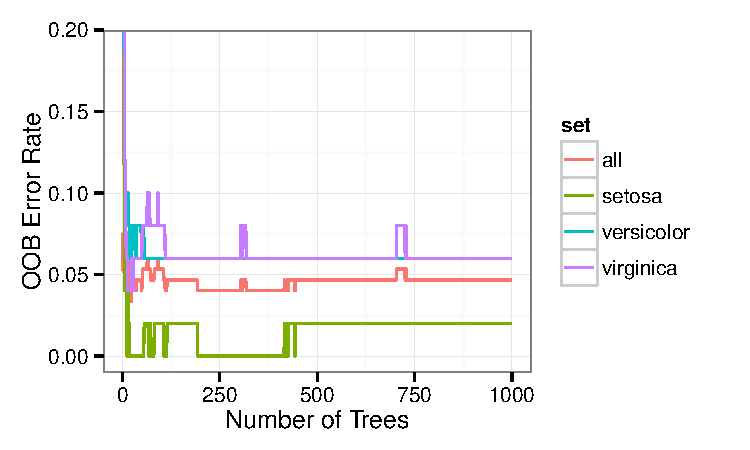
\includegraphics[width=\maxwidth]{figure/vig-iris-rf-error-1} 

}

\caption[Classification Forest]{Classification Forest: Forest error convergence rate.\label{fig:iris-rf-error}}
\end{figure}


\end{knitrout}


\begin{knitrout}\footnotesize
\definecolor{shadecolor}{rgb}{0.969, 0.969, 0.969}\color{fgcolor}\begin{figure}[!htpb]

{\centering 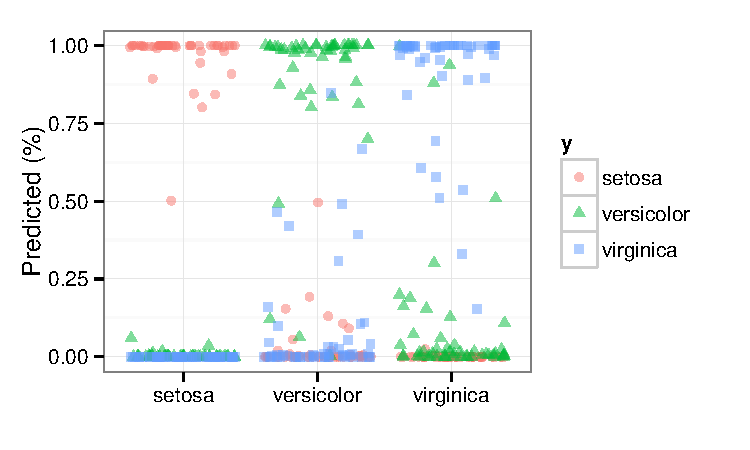
\includegraphics[width=\maxwidth]{figure/vig-iris-rf-pred-1} 

}

\caption[Classification Forest]{Classification Forest: Predicted probability of IRIS class.\label{fig:iris-rf-pred}}
\end{figure}


\end{knitrout}


\begin{knitrout}\footnotesize
\definecolor{shadecolor}{rgb}{0.969, 0.969, 0.969}\color{fgcolor}\begin{figure}[!htpb]

{\centering 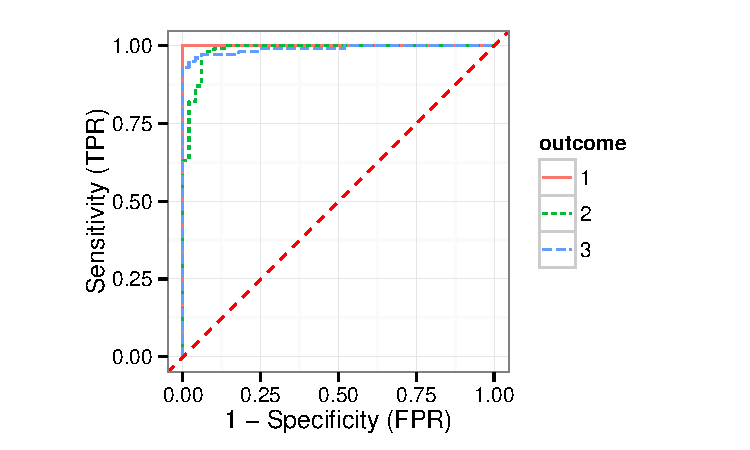
\includegraphics[width=\maxwidth]{figure/vig-iris-rf-roc-1} 

}

\caption[Classification Forest]{Classification Forest: ROC curves.\label{fig:iris-rf-roc}}
\end{figure}


\end{knitrout}

\subsection{Regression Forests}

\begin{knitrout}\footnotesize
\definecolor{shadecolor}{rgb}{0.969, 0.969, 0.969}\color{fgcolor}\begin{kframe}
\begin{verbatim}
R> # Grow the regression forest
R> airq_rf <- rfsrc(Ozone ~ ., data = airquality, na.action = "na.impute")
R> 
R> # Plot the error convergence rate for the forest growth
R> gg_err <- gg_error(airq_rf)
R> plot(gg_err)
R> 
R> # Plot predicted values for the training data
R> gg_rfr <- gg_rfsrc(airq_rf)
R> plot(gg_rfr)
\end{verbatim}
\end{kframe}
\end{knitrout}

% Turn echo=FALSE and res for rfsrc commands...

\begin{knitrout}\footnotesize
\definecolor{shadecolor}{rgb}{0.969, 0.969, 0.969}\color{fgcolor}\begin{kframe}
\begin{verbatim}
                         Sample size: 153
                    Was data imputed: yes
                         Missingness: 27.45%
                     Number of trees: 1000
          Minimum terminal node size: 5
       Average no. of terminal nodes: 17.75
No. of variables tried at each split: 2
              Total no. of variables: 5
                            Analysis: RF-R
                              Family: regr
                      Splitting rule: regr
                % variance explained: 75.55
                          Error rate: 266.1
\end{verbatim}
\end{kframe}\begin{figure}[!htpb]

{\centering 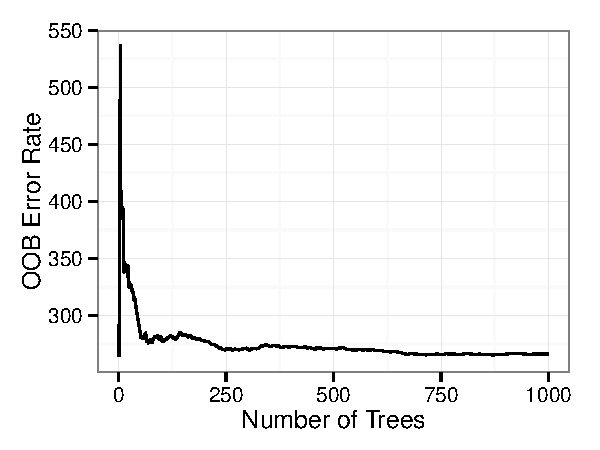
\includegraphics[width=\maxwidth]{figure/vig-airq-rf-error-1} 

}

\caption[Regression forest]{Regression forest:  Forest error convergence rate.\label{fig:airq-rf-error}}
\end{figure}


\end{knitrout}

\begin{knitrout}\footnotesize
\definecolor{shadecolor}{rgb}{0.969, 0.969, 0.969}\color{fgcolor}\begin{figure}[!htpb]

{\centering 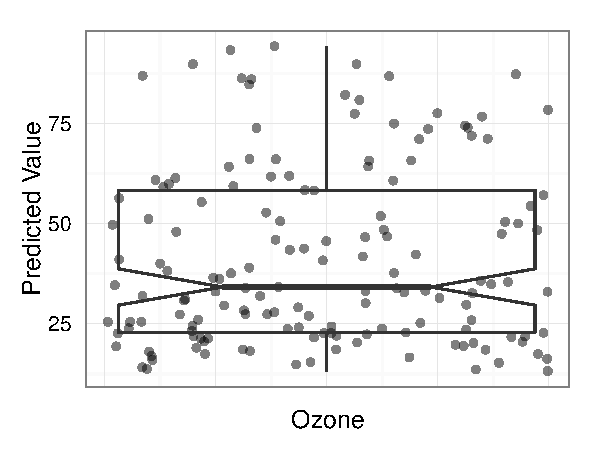
\includegraphics[width=\maxwidth]{figure/vig-airq-rf-plot-1} 

}

\caption[Regression forest]{Regression forest: Predicted Ozone level.\label{fig:airq-rf-plot}}
\end{figure}


\end{knitrout}


\subsection{Survival Forests}
% Turn eval=FALSE for rfsrc commands...
\begin{knitrout}\footnotesize
\definecolor{shadecolor}{rgb}{0.969, 0.969, 0.969}\color{fgcolor}\begin{kframe}
\begin{verbatim}
R> # Load the dataset,
R> data(pbc, package = "randomForestSRC")
R> 
R> # Grow the survival forest
R> pbc_rf <- rfsrc(Surv(days, status) ~ ., pbc, nsplit = 10, ntree=500)
R> 
R> # Plot the error convergence rate for the forest growth
R> plot.gg_error(pbc_rf)
R> 
R> # Plot predicted survival probabilities for the training data
R> plot.gg_rfsrc(pbc_rf) +
+    theme(legend.position=c(.8,.8))
\end{verbatim}
\end{kframe}
\end{knitrout}

% Turn echo=FALSE and res for rfsrc commands...

\begin{knitrout}\footnotesize
\definecolor{shadecolor}{rgb}{0.969, 0.969, 0.969}\color{fgcolor}\begin{kframe}
\begin{verbatim}
                         Sample size: 276
                    Number of deaths: 111
                     Number of trees: 500
          Minimum terminal node size: 3
       Average no. of terminal nodes: 54.39
No. of variables tried at each split: 5
              Total no. of variables: 17
                            Analysis: RSF
                              Family: surv
                      Splitting rule: logrank *random*
       Number of random split points: 10
                          Error rate: 16.42%
\end{verbatim}
\end{kframe}\begin{figure}[!htpb]

{\centering 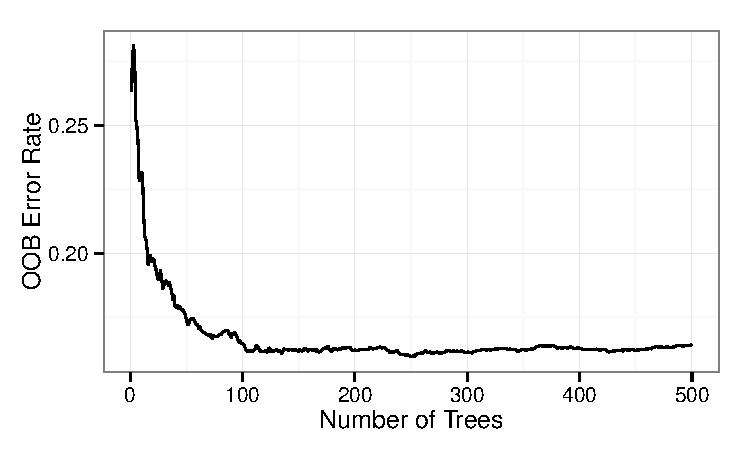
\includegraphics[width=\maxwidth]{figure/vig-surv-rf-error-1} 

}

\caption[Survival Forest]{Survival Forest: Predicted probability of survival.\label{fig:surv-rf-error}}
\end{figure}


\end{knitrout}

\begin{knitrout}\footnotesize
\definecolor{shadecolor}{rgb}{0.969, 0.969, 0.969}\color{fgcolor}\begin{figure}[!htpb]

{\centering 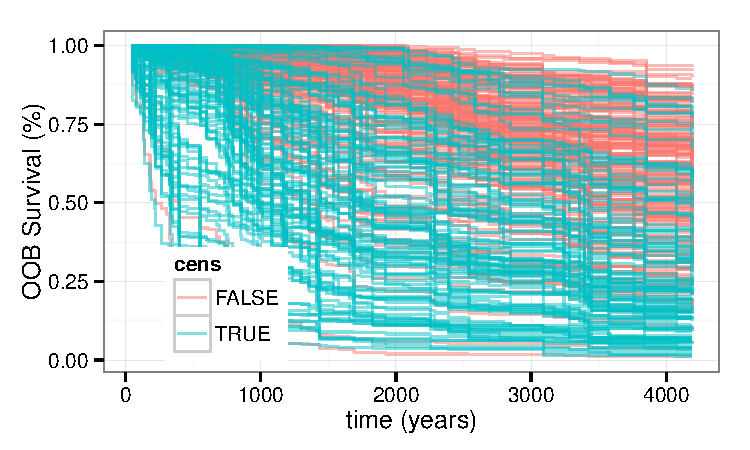
\includegraphics[width=\maxwidth]{figure/vig-surv-rf-plot-1} 

}

\caption[Survival Forest]{Survival Forest: Predicted probability of survival.\label{fig:surv-rf-plot}}
\end{figure}


\end{knitrout}


% -----------------------------------------------------
\section{Identification of Predictive Variables}
% -----------------------------------------------------
Unlike the linear model settings, RF does not explicity specify the functional form of the covariate response relation. We use two seperate methods in order to determine how the RF has built the response prediction, the standard method of Variable Importance (VIMP) as well as the forest minimal depth.


\subsection{Variable Importance}\label{S:vimp}
Variable importance (VIMP) was originally defined in CART using a measure involving surrogate variables (see Chapter 5 of~\cite{cart:1984}). Definitions in terms of mean overall improvement in node impurity for a tree have also been proposed. In regression trees, node impurity is measured by mean squared error, whereas in classification problems, the Gini index is used~\citep{FriedmanGreedyfunction:2000}. The most popular VIMP method to date, however, adopts a prediction error approach involving "noising-up" a variable. In random forests, for example, VIMP for a variable $x_v$ is the difference between prediction error when $x_v$ is noised up by permuting its value randomly, compared to prediction error under the original predictor~\citep{Breiman:2001,liaw:2002,Ishwaran:2007,Ishwaran:2008}.

Given that VIMP is the absolute difference between prediction errors before and after permutation, a large VIMP value indicates that misspecification of that variable detracts from the predictive accuracy of the forest. VIMP close to zero indicates the variable has no impact on predictive accuracy, and negative values indicate the predictive accuracy improves when the variable is mispecified. In the later case, we assume noise is more informative than the variable. As such, we ignore variables with negative and zero values of VIMP, relying on large positive values to indicate that the predictive power of the forest is dependent on those variables. 
\begin{knitrout}\footnotesize
\definecolor{shadecolor}{rgb}{0.969, 0.969, 0.969}\color{fgcolor}\begin{kframe}
\begin{verbatim}
R> plot.gg_vimp(iris_rf)+
+    theme(legend.position="none")
\end{verbatim}
\end{kframe}

{\centering 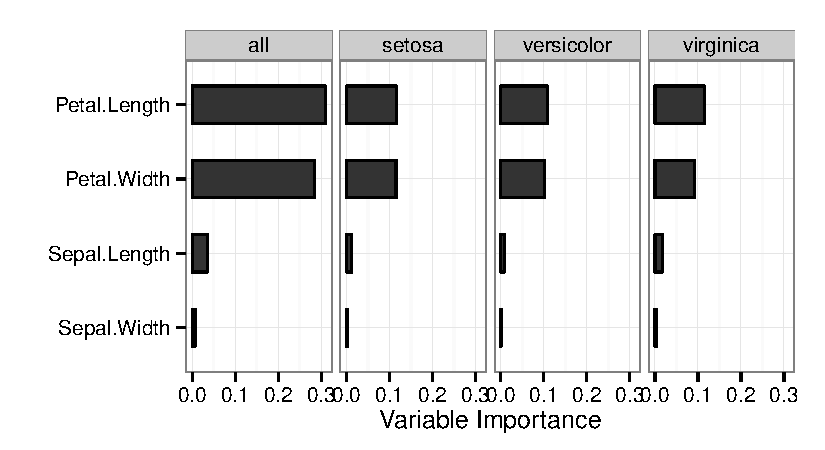
\includegraphics[width=\maxwidth]{figure/vig-iris-vimp-1} 

}



\end{knitrout}

\begin{knitrout}\footnotesize
\definecolor{shadecolor}{rgb}{0.969, 0.969, 0.969}\color{fgcolor}\begin{kframe}
\begin{verbatim}
R> plot.gg_vimp(airq_rf)
\end{verbatim}
\end{kframe}

{\centering 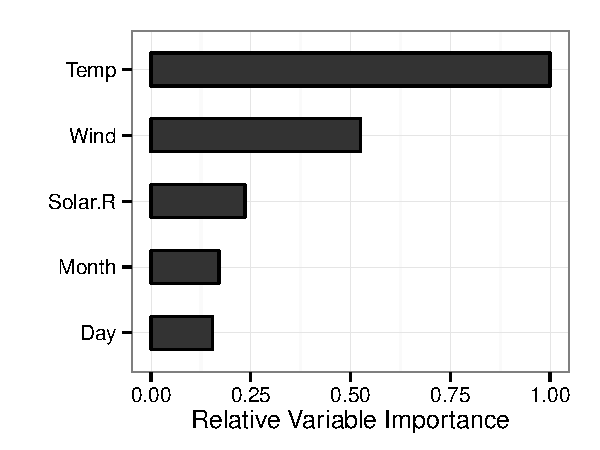
\includegraphics[width=\maxwidth]{figure/vig-airq-vimp-1} 

}



\end{knitrout}

\begin{knitrout}\footnotesize
\definecolor{shadecolor}{rgb}{0.969, 0.969, 0.969}\color{fgcolor}\begin{kframe}
\begin{verbatim}
R> plot.gg_vimp(pbc_rf)+
+    theme(legend.position=c(.8,.2))
\end{verbatim}
\end{kframe}

{\centering 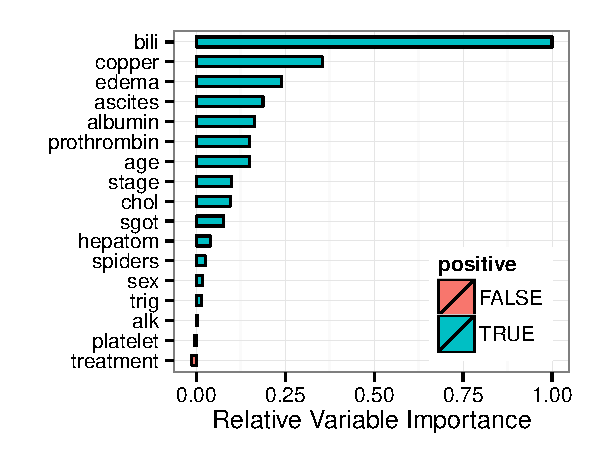
\includegraphics[width=\maxwidth]{figure/vig-pbc-vimp-1} 

}



\end{knitrout}

\subsection{Minimal Depth}\label{S:minimalDepth}
In VIMP, prognostic risk factors are determined by inspection of the forest, ranking the most important variables according to impact on predictive ability of the forest. An alternative method recognizes that most important variables for prediction are those that most frequently split nodes nearest to the trunks of the trees (ie, at the root node). Node levels are numbered based on their relative distance to the trunk of the tree (ie. 0, 1, 2).  A measure of important risk factors is determined by averaging the depth of first split for each variable over all trees within the forest. Lower values of this measure indicate those variables that split larger groups of patients. This method has been shown to successfully identify the strongest predictors, with no loss of overall model accuracy because of excessive parsimony.

The maximal subtree for a variable $x$ is the largest subtree whose root node splits on $x$. Thus, all parent nodes of $x$'s maximal subtree have nodes that split on variables other than $x$. The largest maximal subtree possible is the root node. In general, however, there can be more than one maximal subtree for a variable. A maximal subtree may also not exist if there are no splits on the variable.

The minimal depth of a maximal subtree (the first order depth) measures predictiveness of a variable $x$. It equals the shortest distance (the depth) from the root node to the parent node of the maximal subtree (zero is the smallest value possible). The smaller the minimal depth, the more impact $x$ has on prediction. The mean of the minimal depth distribution is used as the threshold value for deciding whether a variable's minimal depth value is small enough for the variable to be classified as strong. 

% <<iris-mindepth>>=
% plot.gg_minimal_depth(iris_rf)
% @
% 
% <<airq-mindepth>>=
% plot.gg_minimal_depth(airq_rf)
% @

\begin{knitrout}\footnotesize
\definecolor{shadecolor}{rgb}{0.969, 0.969, 0.969}\color{fgcolor}\begin{kframe}
\begin{verbatim}
R> data(pbc_vs, package="ggRandomForests")
R> plot.gg_minimal_depth(pbc_vs)
\end{verbatim}
\end{kframe}

{\centering 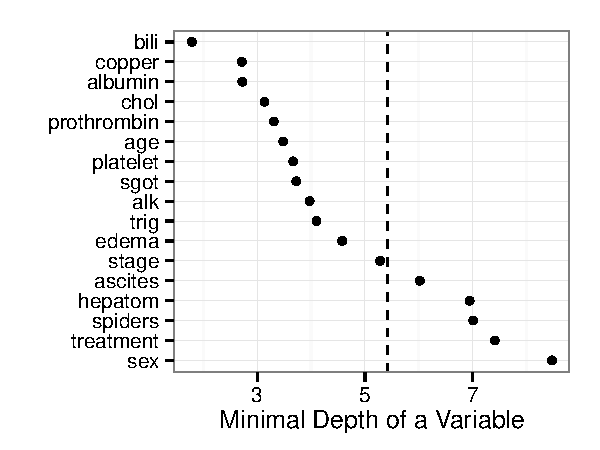
\includegraphics[width=\maxwidth]{figure/vig-pbc-mindepth-1} 

}



\end{knitrout}

\subsection{Variable Importance and Minimal Depth}
\begin{knitrout}\footnotesize
\definecolor{shadecolor}{rgb}{0.969, 0.969, 0.969}\color{fgcolor}\begin{kframe}
\begin{verbatim}
R> plot.gg_minimal_vimp(pbc_rf)
minimal depth variable selection ...


-----------------------------------------------------------
family             : surv 
var. selection     : Minimal Depth 
conservativeness   : medium 
x-weighting used?  : TRUE 
dimension          : 17 
sample size        : 276 
ntree              : 500 
nsplit             : 10 
mtry               : 5 
nodesize           : 3 
refitted forest    : FALSE 
model size         : 12 
depth threshold    : 5.444 
PE (true OOB)      : 16.42 


Top variables:
            depth   vimp
bili        1.754  0.065
copper      2.660  0.023
albumin     2.694  0.011
chol        3.084  0.007
prothrombin 3.228  0.008
age         3.246  0.011
sgot        3.750  0.006
platelet    3.894 -0.001
edema       3.946  0.016
alk         3.988  0.002
trig        4.258  0.000
stage       5.324  0.008
-----------------------------------------------------------
\end{verbatim}
\end{kframe}

{\centering 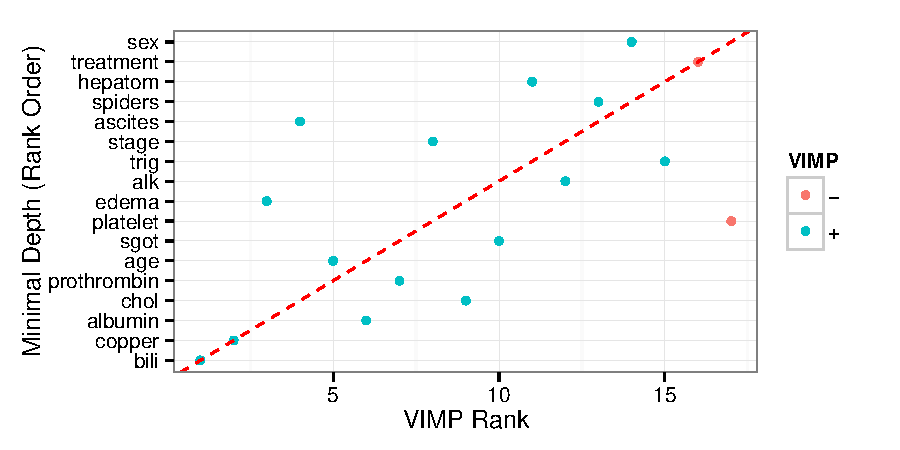
\includegraphics[width=\maxwidth]{figure/vig-pbc-minvimp-1} 

}



\end{knitrout}


\section{Variable Dependence}
Once we have an idea of which variables contribute to the predictive accuracy of the forest, it is useful to get some idea of form of this contribution. We use graphical methods to show the predicted response given dependence on covariates. We can plot the marginal effect of an covariate on the class probability (classification), response (regression), mortality (survival), or the expected years lost (competing risk) for a RF analysis. We plot the ensemble predicted value on the vertical axis and covariates along the horizontal axis.

\subsection{Marginal Dependence}\label{S:variablePlots}
\emph{Marginal variable dependence} plots the predicted response as a function of the covariate, showing each subject as a point on the plot. For classification and regression, this is straight forward predicting the response. In survival settings, we must account for the additional dimension of time. In this case, we plot the response at a specific time point of interest, for example survival at one year. Each predicted point is dependent on the full combination of all covariates, not only on the covariate displayed in the dependence plot. So interpretation can only be in general terms.  
\begin{knitrout}\footnotesize
\definecolor{shadecolor}{rgb}{0.969, 0.969, 0.969}\color{fgcolor}\begin{kframe}
\begin{verbatim}
R> ggrf <- gg_variable(pbc_rf, time=90)
R> 
R> plot(ggrf, x_var = "bili") +
+    theme(legend.position=c(.8,.2))
\end{verbatim}
\end{kframe}

{\centering 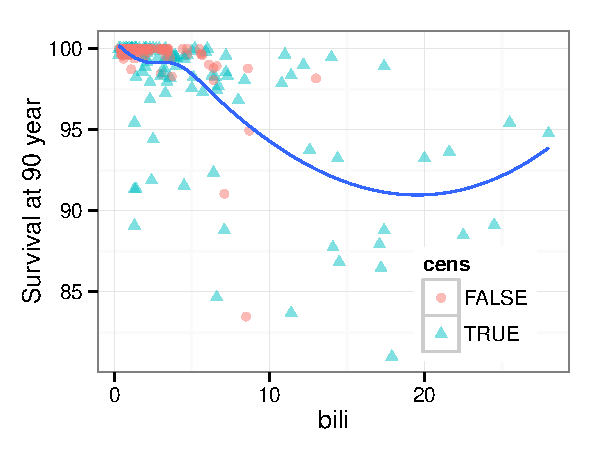
\includegraphics[width=\maxwidth]{figure/vig-variable-plot-1} 

}



\end{knitrout}

\begin{knitrout}\footnotesize
\definecolor{shadecolor}{rgb}{0.969, 0.969, 0.969}\color{fgcolor}\begin{kframe}
\begin{verbatim}
R> ggrf <- gg_variable(pbc_rf, time=c(90,  365, 3*365))
R> 
R> plot(ggrf, x_var = "bili")+
+    scale_shape_manual(values=event.marks, labels=event.labels)+
+    scale_color_manual(values=strCol, na.value="lightgrey", drop=FALSE,
+                       labels=event.labels)
\end{verbatim}
\end{kframe}

{\centering 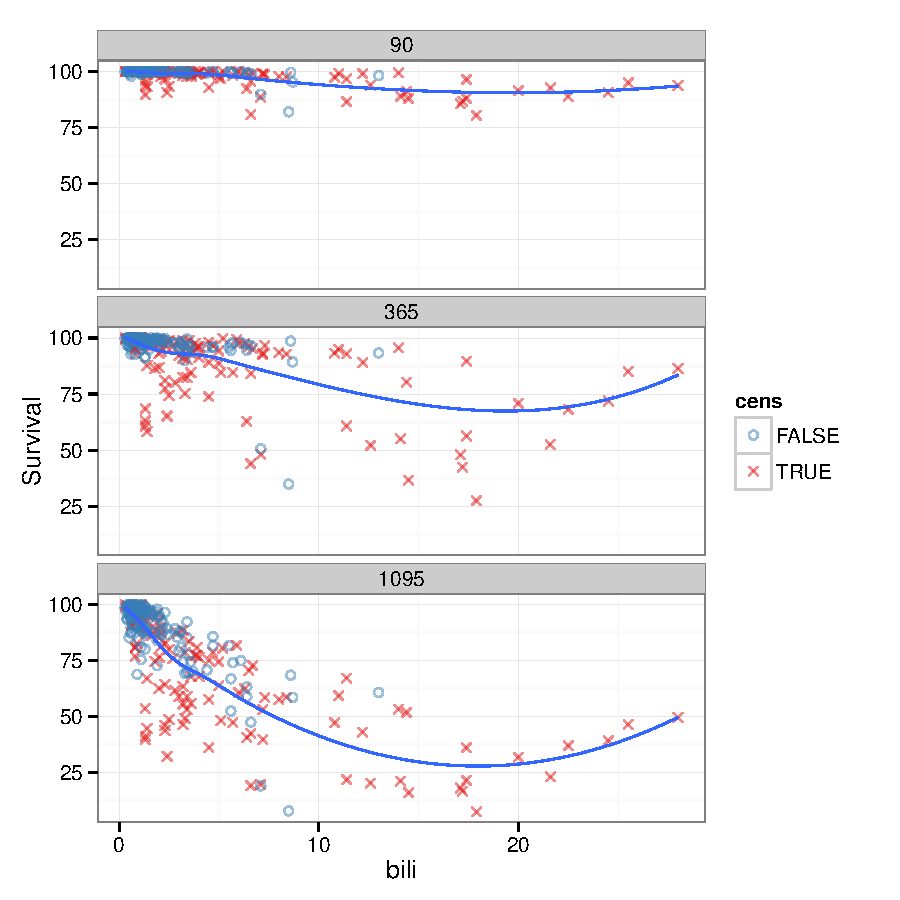
\includegraphics[width=\maxwidth]{figure/vig-variable-plot-stacks-1} 

}



\end{knitrout}

\subsection{Partial Dependence}\label{S:variablePlots}

An alternative to marginal variable dependence is to integrate out the effects of varaibles beside the covariate of interest. For these \emph{partial variable dependence} plots, the y-value for a variable X, evaluated at X=x, is
\[
\tilde{f}(x) = \frac{1}{n} \sum_{i=1}^n \hat{f}(x, x_{i,o}),
\]
where $\hat{f}$ is the predicted response and $x_{i,o}$ represents the value for all other covariates other than $X$ for the observation $i$~\citep{FriedmanGreedyfunction:2000}. The partial plot can be viewed as a risk adjusted estimate of the response as a function of the covariate $X$.

\begin{knitrout}\footnotesize
\definecolor{shadecolor}{rgb}{0.969, 0.969, 0.969}\color{fgcolor}\begin{kframe}
\begin{verbatim}
R> data(pbc_prtl, package="ggRandomForests")
R> ggprtl <- gg_partial(pbc_prtl)
R> 
R> plot(ggprtl[[1]])
\end{verbatim}
\end{kframe}

{\centering 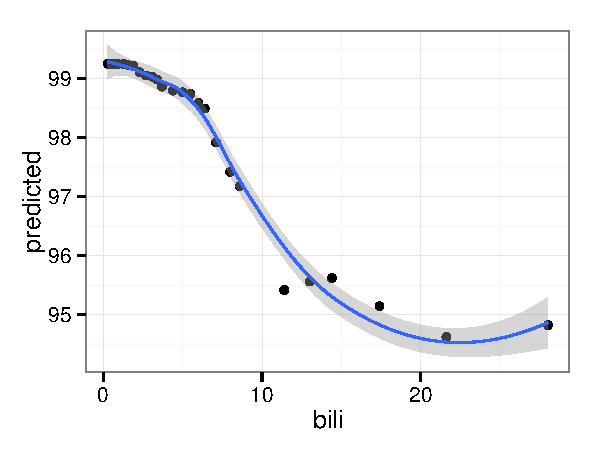
\includegraphics[width=\maxwidth]{figure/vig-pbc-partial-bili-1} 

}



\end{knitrout}

\begin{knitrout}\footnotesize
\definecolor{shadecolor}{rgb}{0.969, 0.969, 0.969}\color{fgcolor}\begin{kframe}
\begin{verbatim}
R> plot(ggprtl[[4]], se=FALSE)
\end{verbatim}
\end{kframe}

{\centering 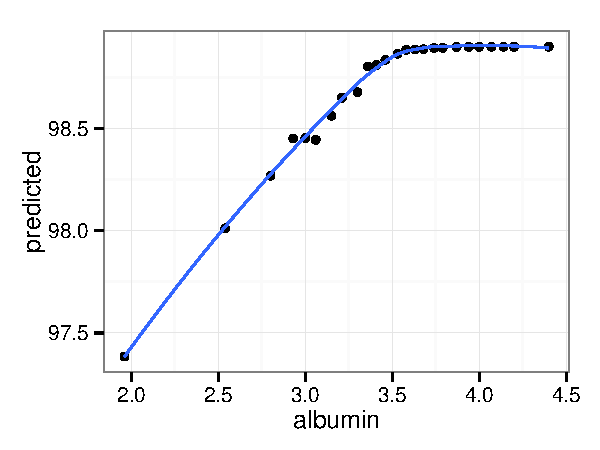
\includegraphics[width=\maxwidth]{figure/vig-pbc-partial-albumin-1} 

}



\end{knitrout}



\subsection{Variable Interactions and Conditional Plots}
Using the different variable dependence measures, we can calculate pairwise interactions for any pair of variables. 

Using minimal depth, we calculate the maximal subtree using the normalized minimal depth of variable $i$ relative to the root node (normalized wrt the size of the tree) the maximal subtree interaction measure  is the normalized minimal depth of a variable $j$ wrt the maximal subtree for variable $i$ (normalized wrt the size of $i$'s maximal subtree). Smaller diagonal entries indicate predictive variables. Small interaction entries having small diagonal entries are a sign of an interaction between variable $i$ and $j$~\citep{Ishwaran_HighDimension:2010,Ishwaran_HighDimension:2011} 

A joint-VIMP approach is also available where two variables are paired and their paired VIMP calculated (refered to as 'Paired' importance). The VIMP for each separate variable is also calculated. The sum of these two values is refered to as 'Additive' importance. A large positive or negative difference between 'Paired' and 'Additive' indicates an association worth pursuing if the univariate VIMP for each of the paired-variables is reasonably large~\citep{Ishwaran:2007}.

By plotting the resulting interaction measures for each variable, we can detect the "most interactive" pairs, and develop conditonal plots~\cite{}. These plots are similar to stratifed results, arranged in a set of panels by the interactive variable of interest. 


\subsection{Variable Interactions}


\subsection{Conditional Dependence}

% =======================================
\section{Conclusions} \label{S:conclusion}
% =======================================


% =======================================
\section{Acknowledgments} \label{S:acknowledge}
% =======================================

% =======================================
% \section{Literatur} \label{sec: references}
% =======================================
%\nocite{*}

\bibliography{ggRandomForests}



\end{document}

% -----------------------------------------------------
\section{Example Datasets}
% -----------------------------------------------------
\subsection{Classification: IRIS}

\subsection{Regression: Air Quality}

\subsection{Regression: Cars}

\subsection{Survival: Veteran}

\subsection{Survival: PBC}


\subsection{Forest Imputation}\label{S:imputation}

The randomForests package~\citep{liaw:2002} include a forest imputation method within the randomForest package. 

We impute missing data (both x and y-variables) using a modification of the missing data algorithm of~\cite{Ishwaran:2008}. Prior to splitting a node, missing data for a variable is imputed by randomly drawing values from non-missing in-bag data. The purpose of the imputed data is to make it possible to assign cases to daughter nodes in the event the node is split on a variable with missing data. Imputed data is however not used to calculate the split-statistic which uses non-missing data only. Following a node split, imputed data are reset to missing and the process is repeated until terminal nodes are reached. Missing data is then imputed using OOB non-missing terminal node data. For integer valued variables and censoring indicators, imputation uses a maximal class rule, whereas continuous variables and survival time use a mean rule.

The proximity matrix from the randomForest is used to update the imputation of the NAs. For continuous predictors, the imputed value is the weighted average of the non-missing obervations, where the weights are the proximities. For categorical predictors, the imputed value is the category with the largest average proximity. This process is iterated iter times.

Regardless of what method is used, records in which all outcome and x-variable information are missing are removed from the forest analysis. Variables having all missing values are also removed.
